% ======================================== Début Préambule Latex ========================================
% Copyright (c) 2022 Mathis Gauthey
% This source code is licensed under the MIT License found in the
% LICENSE file in the root directory of this source tree.

% ========== Classe du document ==========
\documentclass[a4paper,11pt]{report}    % A4, police taille 11, report pour avoir les chapitres

% ============ Vista 
\usepackage{paracol}
%%% -----------------------------------------------------------------------------
%% 2017 por Fausto M. Lagos S. <piratax007@protonmail.ch>
%% 
%% Este trabajo puede ser distribuido o modificado bajo los
%% términos y condiciones de la LaTeX Project Public License (LPPL) v1.3C, 
%% o cualquier versión posterior. La última versión de esta licencia
%% puede verse en:
%% http://www.latex-project.org/lppl.txt
%% 
%% -----------------------------------------------------------------------------
%% Usted es libre de usarlo, modificarlo o distribuirlo siempre que se
%% respeten los términos de la licencia y se reconozca al autor original.
%% -----------------------------------------------------------------------------

\usepackage{xcolor}
\usepackage{tcolorbox}
\tcbuselibrary{listings, skins}
\usepackage{listings}

\definecolor{arduino}{HTML}{00A3A9}
\definecolor{structure}{HTML}{818A42}
\definecolor{variables}{HTML}{128F8F}
\definecolor{functions}{HTML}{DB6B21}
\definecolor{back}{HTML}{E0E0E2}
\definecolor{myblue}{rgb}{0.01,0.61,0.98}
\definecolor{mygray}{rgb}{0.47,0.47,0.33}

\newcommand*{\FormatDigit}[1]{\ttfamily\textcolor{black}{#1}}
%% http://tex.stackexchange.com/questions/32174/listings-package-how-can-i-format-all-numbers
\lstdefinestyle{FormattedNumber}{%
    literate=*{0}{{\FormatDigit{0}}}{1}%
             {1}{{\FormatDigit{1}}}{1}%
             {2}{{\FormatDigit{2}}}{1}%
             {3}{{\FormatDigit{3}}}{1}%
             {4}{{\FormatDigit{4}}}{1}%
             {5}{{\FormatDigit{5}}}{1}%
             {6}{{\FormatDigit{6}}}{1}%
             {7}{{\FormatDigit{7}}}{1}%
             {8}{{\FormatDigit{8}}}{1}%
             {9}{{\FormatDigit{9}}}{1}%
             {.0}{{\FormatDigit{.0}}}{2}% 
             {.1}{{\FormatDigit{.1}}}{2}% 
             {.2}{{\FormatDigit{.2}}}{2}%
             {.3}{{\FormatDigit{.3}}}{2}%
             {.4}{{\FormatDigit{.4}}}{2}%
             {.5}{{\FormatDigit{.5}}}{2}%
             {.6}{{\FormatDigit{.6}}}{2}%
             {.7}{{\FormatDigit{.7}}}{2}%
             {.8}{{\FormatDigit{.8}}}{2}%
             {.9}{{\FormatDigit{.9}}}{2}%
             %{,}{{\FormatDigit{,}}{1}% Eliminar el comentario si quiere "," en color
             {\ }{{ }}{1}%
             ,%
}

\lstset{%
  basicstyle=\footnotesize,       
  breakatwhitespace=false,         
  breaklines=true,                 
  captionpos=b,                   
  commentstyle=\color{gray},    
  deletekeywords={...},           
  escapeinside={\%*}{*)},          
  extendedchars=true,              
  keepspaces=true,                 
  keywordstyle=[1]\color{structure},
  keywordstyle=[2]\color{variables},
  keywordstyle=[3]\color{functions},
  keywordstyle=[4]\bfseries\color{functions},
  language=c++,                
  morekeywords={*,...},     
  numbers=left,                    
  numbersep=5pt,                   
  numberstyle=\tiny\color{mygray}, 
  rulecolor=\color{black},         
  rulesepcolor=\color{myblue},
  showspaces=false,                
  showstringspaces=false,          
  showtabs=false,                
  stringstyle=\color{rgb: red,0.33;green,0.45;blue,0.87},    
  tabsize=2,                       
  title=\lstname,
  emphstyle=\color{variables},
  frame = single,
  framexleftmargin = 15pt,
  rulecolor = \color{arduino},
}

\lstdefinestyle{Arduino}{%
    style=FormattedNumber,
    keywords={setup, loop, if, else, for, switch, while, do, break, continue, return, goto},
    morekeywords=[2]{HIGH, LOW, INPUT, OUTPUT, INPUT_PULLUP, LED_BUILTIN, true, false, int, float, void, boolean, char, word, long, short, double, string, array},
    morekeywords=[3]{const, pinMode, digitalWrite, digitalRead, analogReference, analogRead, analogWrite, analogReadResolution, analogWriteResolution, tone, noTone, shiftOut, shiftIn, pulseIn, millis, micros, delay, delayMicroseconds, min, max, abs, constrain, map, pow, sqrt, sin, cos, tan, isAlphaNumeric, inAlpha, isAscii, isWhitespace, isControl, isDigit, isGraph, isLowerCase, isPintable, isPunct, isSpace, isUpperCase, isHexadecimalDigit, randomSeed, random, lowByte, highByte, bitRead, bitWrite, bitSet, bitClear, bit, attachInterrupt, detachInterrupt, interrupts, noInterrupts, Stream, Keyboard, Mouse, begin, println, print},
    morekeywords=[4]{Serial},
    morecomment=[l]{//},
    morecomment=[s]{/*}{*/},
    emph={const},
}

% Comando para incluir un sketch de Arduino, el primer parámetro es el nombre del archivo que contiene el script (sin .ino), el segundo es el etiqueta del contador Listing
\newcommand{\ArduinoSketch}[2]{
\begin{itemize}
\item[]\lstinputlisting[caption=#2,label=#1,style=Arduino]{#1.ino}
\end{itemize}
}

% Ambiente para incluir un sketch de Arduino escribiendo el código directamente en el documento LaTeX, tiene un parámetro de entrada que corresponde al título del sketch
\newtcblisting{ArduinoSketchBox}[2][colframe = arduino, enhanced, drop shadow, hbox]{
	arc = 3pt, outer arc = 3pt,
	listing only,
	listing options = {
		frame =,
		style = Arduino,
	},
	title = #2,
	#1
}
%-----------------------------------------------------------------------------


\usepackage{xcolor}
\usepackage{tcolorbox}
\tcbuselibrary{listings, skins}
\usepackage{listings}
\usepackage{caption}

\definecolor{arduino}{HTML}{00A3A9}
\definecolor{structure}{HTML}{818A42}
\definecolor{variables}{HTML}{128F8F}
\definecolor{functions}{HTML}{DB6B21}
\definecolor{back}{HTML}{E0E0E2}
\definecolor{myblue}{rgb}{0.01,0.61,0.98}
\definecolor{mygray}{rgb}{0.47,0.47,0.33}

\newcommand*{\FormatDigit}[1]{\ttfamily\textcolor{black}{#1}}
%% http://tex.stackexchange.com/questions/32174/listings-package-how-can-i-format-all-numbers
\lstdefinestyle{FormattedNumber}{%
    literate=*{0}{{\FormatDigit{0}}}{1}%
             {1}{{\FormatDigit{1}}}{1}%
             {2}{{\FormatDigit{2}}}{1}%
             {3}{{\FormatDigit{3}}}{1}%
             {4}{{\FormatDigit{4}}}{1}%
             {5}{{\FormatDigit{5}}}{1}%
             {6}{{\FormatDigit{6}}}{1}%
             {7}{{\FormatDigit{7}}}{1}%
             {8}{{\FormatDigit{8}}}{1}%
             {9}{{\FormatDigit{9}}}{1}%
             {.0}{{\FormatDigit{.0}}}{2}% 
             {.1}{{\FormatDigit{.1}}}{2}% 
             {.2}{{\FormatDigit{.2}}}{2}%
             {.3}{{\FormatDigit{.3}}}{2}%
             {.4}{{\FormatDigit{.4}}}{2}%
             {.5}{{\FormatDigit{.5}}}{2}%
             {.6}{{\FormatDigit{.6}}}{2}%
             {.7}{{\FormatDigit{.7}}}{2}%
             {.8}{{\FormatDigit{.8}}}{2}%
             {.9}{{\FormatDigit{.9}}}{2}%
             %{,}{{\FormatDigit{,}}{1}% Eliminar el comentario si quiere "," en color
             {\ }{{ }}{1}%
             ,%
}

\lstset{%
  basicstyle=\footnotesize,       
  breakatwhitespace=false,         
  breaklines=true,                 
  captionpos=b,                   
  commentstyle=\color{gray},    
  deletekeywords={...},           
  escapeinside={\%*}{*)},          
  extendedchars=true,              
  keepspaces=true,                 
  keywordstyle=[1]\color{structure},
  keywordstyle=[2]\color{variables},
  keywordstyle=[3]\color{functions},
  keywordstyle=[4]\bfseries\color{functions},
  language=c++,                
  morekeywords={*,...},     
  numbers=left,                    
  numbersep=5pt,                   
  numberstyle=\tiny\color{mygray}, 
  rulecolor=\color{black},         
  rulesepcolor=\color{myblue},
  showspaces=false,                
  showstringspaces=false,          
  showtabs=false,                
  stringstyle=\color{rgb: red,0.33;green,0.45;blue,0.87},    
  tabsize=2,                       
  title=\lstname,
  emphstyle=\color{variables},
  frame = single,
  framexleftmargin = 15pt,
  rulecolor = \color{arduino},
}

\lstdefinestyle{Arduino}{%
    style=FormattedNumber,
    keywords={setup, loop, if, else, for, switch, while, do, break, continue, return, goto},
    morekeywords=[2]{HIGH, LOW, INPUT, OUTPUT, INPUT_PULLUP, LED_BUILTIN, true, false, int, float, void, boolean, char, word, long, short, double, string, array},
    morekeywords=[3]{const, pinMode, digitalWrite, digitalRead, analogReference, analogRead, analogWrite, analogReadResolution, analogWriteResolution, tone, noTone, shiftOut, shiftIn, pulseIn, millis, micros, delay, delayMicroseconds, min, max, abs, constrain, map, pow, sqrt, sin, cos, tan, isAlphaNumeric, inAlpha, isAscii, isWhitespace, isControl, isDigit, isGraph, isLowerCase, isPintable, isPunct, isSpace, isUpperCase, isHexadecimalDigit, randomSeed, random, lowByte, highByte, bitRead, bitWrite, bitSet, bitClear, bit, attachInterrupt, detachInterrupt, interrupts, noInterrupts, Stream, Keyboard, Mouse, begin, println, print},
    morekeywords=[4]{Serial},
    morecomment=[l]{//},
    morecomment=[s]{/*}{*/},
    emph={const},
}

% Comando para incluir un sketch de Arduino, el primer parámetro es el nombre del archivo que contiene el script (sin .ino), el segundo es el etiqueta del contador Listing
\newcommand{\ArduinoSketch}[2]{
\begin{itemize}
\item[]\lstinputlisting[caption=#2,label=#1,style=Arduino]{#1.ino}
\end{itemize}
}

% Ambiente para incluir un sketch de Arduino escribiendo el código directamente en el documento LaTeX, tiene un parámetro de entrada que corresponde al título del sketch
\newtcblisting{ArduinoSketchBox}[2][colframe = arduino, enhanced, drop shadow, hbox]{
	arc = 3pt, outer arc = 3pt,
	listing only,
	listing options = {
		frame =,
		style = Arduino,
	},
	title = #2,
	#1
}

% Entorno para códigos largos
\newenvironment{longlisting}{\captionsetup{type=listing}}{}
% Cambia el nombre del índice de códigos
\renewcommand\lstlistingname{Código}
\renewcommand\lstlistlistingname{Índice de Códigos}
%-----------------------------------------------------------------------------



% ========== Langue française pour le document ==========
\usepackage{latexsym}       % Police latex de base
\usepackage[spanish]{babel}  % Dictionnaire français (indentation, caractères spéciaux, tirets...)
\usepackage[utf8]{inputenc} % Encodage d'entrée pour les caractères accentués
\usepackage[T1]{fontenc}    % Affichage correct des caractères accentués notamment

% ========== Géométrie du document ==========
% Gestion des différentes marges du document pour coller avec le séparateur d'en-tête
\usepackage[left=2cm , right=2cm, bottom=2cm, top=2cm, headheight=2cm, headsep=0.5cm,heightrounded=true]{geometry}
% \raggedbottom % This makes the last line of each page be at exactly the same place on the sheet of paper
% \flushbottom  % All pages will not necessarily have exactly the same height, but ‘almost the same height’
\setlength{\parskip}{1em}   % Définition de l'espace entre les paragraphes
\setlength{\parindent}{4em} % Définition de la longueur du "tab" = indentation
\usepackage{fancyhdr}       % Permet en-tête et pied de page
\pagestyle{fancyplain}      % Pour avoir le même style sur les pages fancy et sur celles plains comme la toc
\renewcommand\plainheadrulewidth{.4pt}  % Le trait noir sous les logos sur les pages plain
\fancyhead[L]{
\includegraphics[scale=0.3]{IPN.png}}    % Logo gauche
\fancyhead[R]{
\includegraphics[scale=0.2]{upiir.png}} % Logo droit
% Redéfinir le style "empty" utilisé par le documentclass "report" pour le titre, résumé et chapitres
\fancypagestyle{empty}
{
    \fancyhf{}
    \fancyhead[L]{
\includegraphics[scale=0.3]{IPN.png}}    % Logo gauche
    \fancyhead[R]{
\includegraphics[scale=0.2]{upiir.png}} % Logo droit
}

% ========== Liens dans le document, méta-datas et références ==========
\usepackage{xpatch}     % Permet de patcher certaines fonctionnalités de base comme la toc
\usepackage{float}      % Placement des flottants
\usepackage{hyperref}   % Liens dans le documents
\usepackage{caption}    % Légendes dans les environnements "figure" et "float"
\usepackage[list=true]{subcaption} % Légendes pour les "sous-figures" et "sous-float"
                                   % et affichage des "sous-..." dans la liste des figures
\def\thechapter{\Alph{chapter}}    % Définition des chapitres avec une lettre
\setcounter{tocdepth}{3}           % Profondeur de numérotation de la toc  (chap > sec > subsec > subsubsec)
\setcounter{secnumdepth}{3}        % Profondeur de numérotation des titres (chap > sec > subsec > subsubsec)
\usepackage{chngcntr}              % Permet de changer les numérotations d'objets
\usepackage[titles]{tocloft}       % Gestion très précise des différentes listes

\hypersetup % Attribution des méta-datas pdf pour reconnaissance automatique Zotero entre autres
{
pdftitle={Titre},
pdfsubject={Sujet},
pdfauthor={Auteur},
pdfkeywords={keyword1} {keyword2} {keyword3}
}

% ========== Graphique, police, maths ==========
\usepackage[table,xcdraw]{xcolor}       % Package permettant d'utiliser de la couleur
% \usepackage{color}                      % Rajouter de la couleur au texte
\usepackage{bm}                         % Mettre en gras des maths avec la commande \bm
\usepackage{ragged2e}                   % Meilleure gestion de l'alignement des textes entre autres
\usepackage{tcolorbox}                  % Boite colorées pour texte, images ou équations
\usepackage{textcomp}                   % Symboles et polices
\usepackage{gensymb}                    % Symbole pour le degré entre autre
\usepackage{amsmath,amsfonts,amssymb}   % Écrire des maths
\usepackage{cancel}                     % Barrer des maths
\usepackage{mathtools}                  % Gestion des matrices et de maths complexes
\usepackage{morewrites}                 % Résoud un problème entre les listes équation et codes
%\usepackage[color={[RGB]{255,191,191}}, text=Confidentiel, scale=1]{draftwatermark} % Ajout filigrane

\usepackage{lmodern}
\usepackage[Lenny]{fncychap}

\ChNameUpperCase
\ChNumVar{\fontsize{40}{42}\usefont{OT1}{ptm}{m}{n}\selectfont}
\ChTitleVar{\Huge \bfseries}

\usepackage{pifont}
\usepackage{enumitem}       % Gestion des énumérations

% Gestion des espaces avant et après les listes plus agréable à la vue
% \setlist[itemize]{noitemsep, topsep=5pt, before={\vspace*{-\baselineskip}}}
% Si désactivé (commenté), penser à ajouter un \smallskip, \medskip ou \bigskip après un itemize.

\definecolor{bulletcolor}{RGB}{128,128,128}

\setenumerate[1]{label=\Alph*.}
\setenumerate[2]{label=\arabic*.}
\setenumerate[3]{label=\roman*.}

\setitemize[1]{label=\ding{222}, font=\LARGE \color{bulletcolor}}
\setitemize[2]{label=\textbullet, font=\LARGE \color{bulletcolor}}
\setitemize[3]{label=$\triangleright$, font=\LARGE \color{bulletcolor}}

\usepackage{siunitx}                                    % Pour des unités bien écrites
\newcommand{\nomunit}[1]{%
\renewcommand{\nomentryend}{\hspace*{\fill}#1}}         % Commande pour la nomenclature (unités à droite)
\sisetup{inter-unit-product =\ensuremath{{}\cdot{}}}    % Séparation par un point des unités
\DeclareSIUnit\bar{bar}                                 % Besoin de déclarer les bar car pas pris en charge
\DeclareSIPower\quartic\tothefourth{4}

\usepackage{contour}
\usepackage[normalem]{ulem}

\renewcommand{\ULdepth}{1.8pt}
\contourlength{0.8pt}

\newcommand{\myuline}[1]{%
	\uline{\phantom{#1}}%
	\llap{\contour{white}{#1}}%
}

% myuline on each word to allow linebreaks
\RequirePackage{xparse}
\ExplSyntaxOn
\NewDocumentCommand{\myulineX}{m}
{
	\seq_set_split:Nnn \l_tmpa_seq { ~ } { #1 }
	\seq_map_inline:Nn \l_tmpa_seq { \myuline{##1} ~ } \unskip
}
\ExplSyntaxOff

% ========== Glossaire ==========
\usepackage[acronym,toc]{glossaries}    % Gestion d'un glossaire et d'une liste d'acronymes,
                                        % et ajout dans la toc de la position de ces derniers
% Pas besoin de points à la fin du document

\newglossaryentry{mot_complexe}{
    name={mot complexe},
    description={Un mot complexe nécessite généralement une explication}}

\newacronym{lfala}{LFALA}{Les Français Aiment Les Acronymes}                        % Récupère les informations du fichier glossary.tex
\makeglossaries                         % Génère le glossaire avec les informations récupérées

% ========== Nomenclature ==========
\usepackage[intoc]{nomencl}         % Gestion d'une nomenclature avec position dans la toc
\makenomenclature                   % Génère la nomenclature
\usepackage{etoolbox}               % Permet de créer des groupes de nomenclature

% Création de groupes de nomenclature : ATTENTION -> Uniquement des caractères uniques en identifiant
\renewcommand\nomgroup[1]{%
  \item[\bfseries
  \ifstrequal{#1}{A}{Groupe 1}{%
  \ifstrequal{#1}{B}{Groupe 2}{%
  \ifstrequal{#1}{C}{Groupe 3}{%
  }}}%
]} % Attention aux accolades lors de la création de groupes

\AtBeginDocument{   % Nomenclature à générer
\nomenclature[A]{$c_{air}$}{Célérité du son dans l'air à \SI{15}{\celsius} \nomunit{\SI{340.29}{\meter\per\second}}}
\nomenclature[B]{$T_N$}{Période propre de l'élément considéré}
\nomenclature[B]{\(E\)}{{Module d'Young}}
\nomenclature[C]{$\dot{\epsilon}$}{Vitesse de déformation \nomunit{\si{\per\second}}}
}

% ========== Gestion des figures ==========
\usepackage{graphicx}               % Plus d'arguments pour la fonction \includegraphics
\graphicspath{{Images/}}            % Path des images

\counterwithin{figure}{section}     % Numérotation des figures à partir des sections
\setcounter{lofdepth}{2}            % Afficher jusqu'aux sous-figures dans la liste des figures
\cftsetindents{figure}{0em}{3.5em}  % Réglage de l'espace entre le numéro et le nom de la figure dans la liste
\setlength\cftbeforefigskip{5pt}    % Réglage de l'espacement entre les figures dans la liste
\AtBeginDocument{\renewcommand{\listfigurename}{Índice de figuras}} % Renommer la liste des figures
% Ajout de la position de la liste des figures dans la toc
\xpretocmd{\listoffigures}{\addcontentsline{toc}{chapter}{\listfigurename}}{}{}

% ========== Gestion des tableaux ==========
\usepackage{array,multirow,makecell}                        % Packages utiles pour les tableaux
\setcellgapes{1pt}                                          % Paramètres sympa d'après Xm1Math
\makegapedcells                                             % Paramètres sympa d'après Xm1Math
\newcolumntype{R}[1]{>{\raggedleft\arraybackslash }b{#1}}   % Paramètres sympa d'après Xm1Math
\newcolumntype{L}[1]{>{\raggedright\arraybackslash }b{#1}}  % Paramètres sympa d'après Xm1Math
\newcolumntype{C}[1]{>{\centering\arraybackslash }b{#1}}    % Paramètres sympa d'après Xm1Math

\counterwithin{table}{section}      % Numérotation des tableaux à partir des sections
\setcounter{lotdepth}{2}            % Afficher jusqu'aux sous-tableaux dans la liste des tableaux
\cftsetindents{table}{0em}{3.5em}   % Réglage de l'espace entre le numéro et le nom du tableau dans la liste
\setlength\cftbeforetabskip{5pt}    % Réglage de l'espacement entre les figures dans la liste
% Ajout de la position de la liste des tableaux dans la toc
\xpretocmd{\listoftables}{\addcontentsline{toc}{chapter}{\listtablename}}{}{}

% ========== Gestion des équations ==========
\newcommand{\listequationsname}{Índice de ecuaciones}    % Renommer la liste des équations
\newlistof{myequations}{equ}{\listequationsname}
\newcommand{\myequations}[1]{%
   \addcontentsline{equ}{myequations}{\protect\numberline{\theequation}#1}
}
\counterwithin{equation}{section}           % Numérotation des équations à partir des sections
\cftsetindents{myequations}{0em}{3.5em}     % Réglage de l'espace entre le numéro et le nom de l'équation dans la liste
\setlength\cftbeforemyequationsskip{5pt}    % Réglage de l'espacement entre les équations dans la liste

% Création de la commande \noteworhty pour les équations importantes qui méritent d'être listées
\newcommand{\noteworthy}[2]{
\begin{align} \label{#2} \ensuremath{\boxed{#1}} \end{align}
\myequations{#2}
\begingroup
\centering \small \textit{#2}

\endgroup}

\makeatletter   % Espacement des équations plus important entre les chapitres
\xpretocmd{\@chapter}{\addtocontents{equ}{\protect\addvspace{10\p@}}}{}{}{}%
\makeatother
% Ajout de la position de la liste des équation dans la toc
\xpretocmd{\listofmyequations}{\addcontentsline{toc}{chapter}{\listequationsname}}{}{}

% ========== Gestion des codes ==========
%\usepackage[newfloat]{minted}       % Package permettant d'intégrer du code
% Mode printer friendly
%\usemintedstyle{emacs}            	% Sélection du style de syntaxe
%\definecolor{bg}{HTML}{FFFFFF}      % Définition de la couleur d'arrière plan blanc
% Mode pdf only
%\usemintedstyle{monokai}            % Sélection du style de syntaxe
%\definecolor{bg}{HTML}{282828}      % Définition de la couleur d'arrière plan monokai
%\counterwithin{listing}{section}    % Numérotation des codes à partir des sections

% Configuration de newfloat pour que tout roule
%\newenvironment{code}{\captionsetup{type=listing}}{}
%\SetupFloatingEnvironment{listing}{%
  %name={Listing},
  %fileext=lol}
%\SetupFloatingEnvironment{listing}{listname=Liste des codes}    % Renommer la liste des codes

% Gérer les codes de plus d'une page de document
%\tcbuselibrary{listings, skins}
%\usepackage{listings}
%\usepackage{caption} % Agrega el paquete caption
%\newenvironment{longlisting}{\captionsetup{type=listing}}{} % longlisting pour les codes qui dépassent d'une page
%\vbadness=\maxdimen    % Casse les couilles ya pas de fix qui garde une couleur de background et une bonne liste
                       % du-coup je décide de supprimer les warnings.
% Source : https://tex.stackexchange.com/questions/50830/do-i-have-to-care-about-bad-boxes/50850#50850
%        & https://tex.stackexchange.com/questions/138/what-are-underfull-hboxes-and-vboxes-and-how-can-i-get-rid-of-them

%\setminted          % Paramètre du code standard
%{
%bgcolor=bg,
%frame=lines,
%framesep=2mm,
%baselinestretch=1.2,
%fontsize=\footnotesize,
%linenos=true,
%autogobble
%}
%
%\setmintedinline    % Paramètres du code inline
%{
%bgcolor=bg,
%frame=lines,
%framesep=2mm,
%baselinestretch=1.2,
%fontsize=\footnotesize,
%linenos=true,
%autogobble
%}

% ========== Index ==========
\usepackage{imakeidx}   % Package pour créer l'index
\makeindex              % Génération de l'index
% Ajout de la position de l'index dans la toc
\xpretocmd{\printindex}{\addcontentsline{toc}{chapter}{\indexname}}{}{}

% ========== Bibliographie ==========
% Importer un fichier biblatex, sans dépassement des marges, trié par ordre d'apparition
\usepackage[block=ragged,sorting=none]{biblatex}
\usepackage{csquotes}           % Gestion des caractères " " lors des citations
\addbibresource{biblio.bib}     % Importer le fichier de bibliographie
\nocite{*}                      % Importer les éléments non cités quand même dans la bibliographie

% ========== Gestion des annexes ==========
\usepackage[toc,page,title,titletoc,header]{appendix}   % Packages indexes importants
\usepackage{pdfpages}                                   % Intégration de pdf dans le document
\renewcommand{\appendixtocname}{Tabla de anexos}      % Nom de la table des annexes dans la toc
\renewcommand{\appendixpagename}{Anexos}               % Nom du titre de la page des annexes
\usepackage{titletoc}	% Permet de générer une petite table des annexes

% ========== Utilitaires ==========
\usepackage[all,defaultlines=3]{nowidow}    % Macro pour la gestion des lignes seules en bout de page
\usepackage{blindtext}                      % Génération de texte aléatoire pour les exemples
% A utiliser avec https://ctan.mirror.garr.it/mirrors/ctan/macros/latex/contrib/mwe/mwe.pdf pour les images

% ======================================== Fin Préambule Latex ========================================

% ======================================== Début TUTOs ========================================

% ========== Intégrer une image ==========
%\begin{figure}[htbp]
%\centering
%\includegraphics[width=\textwidth]{example-image-a.png}
%\caption{Image A}
%\label{fig:example-image-a} % Bon réflexe de garder le même nom de fichier et de label
%\end{figure}

% ========== Insérer de multiples images ==========
% \begin{figure}[H]
%     \begin{subfigure}[t]{0.475\textwidth}
%         \includegraphics[width=1\textwidth]{example-image-b}
%         \caption{Image B}
%         \label{subfig:example-image-b}
%     \end{subfigure}%
%     ATTENTION, le % est très important ici pour éviter les problèmes de vide
%     \hfill    % Remplissage entre les images
%     \begin{subfigure}[t]{0.475\textwidth}
%         \includegraphics[width=1\textwidth]{example_image_c}
%         \caption{Image C}
%         \label{subfig:example-image-c}
%     \end{subfigure}
%     \caption{Exemple d'utilisation des sous-figures}
%     \label{fig:test_subfigure}
% \end{figure}

% ========== Placement des images ==========
% h Place the float here, i.e., approximately at the same point it occurs in the source text (however, not exactly at the spot)
% t Position at the top of the page.
% b Position at the bottom of the page.
% p Put on a special page for floats only.
% ! Override internal parameters LATEX uses for determining "good" float positions.
% H Places the float at precisely the location in the LATEX code. Requires the float package (\usepackage{float}). This is somewhat equivalent to h!, though some errors may arise if you have too many consecutive floats with [H].

% ========== Intégrer un tableau ==========
% https://www.tablesgenerator.com/

% ========== Intégrer une équation ==========
% https://editor.codecogs.com/
% \noteworthy{equation}{légende} pour l'avoir dans la liste des équations

% ========== Intégrer du code ==========
% \begin{listing}[htbp]
% \begin{minted}{c}
% #include <stdio.h>
% int main() {
%   printf("Hello, World!"); /*printf() outputs the quoted string*/
%   return 0;
% }
% \end{minted}
% \caption{Hello World in C}
% \label{listing:2}
% \end{listing}

% \mint{python}|print("hello")| % Équivalent de \minted mais plus court

% \mintinline{python}|print("hello")|   % Quand t'as qu'une ligne de code

% Remarque : Le séparateur aurait pu être { } ou d'autres ponctuations

% \inputminted[firstline=2, lastline=12]{octave}{BitXorMatrix.m}

% ========== Début de doc classique ==========
% \title{Titre}
% \author{Auteur}
% \date{\today}
% \maketitle
% \begin{abstract}
%     Blablabla
% \end{abstract}

% ======================================== Fin TUTOs ========================================

\begin{document}

% ======================================== Début Page de Garde ========================================

\hypersetup{pageanchor=false}
\begin{titlepage}
    \begin{center}
        \vspace*{1cm}

        \Huge
        \textbf{Curso Diseño de Seguidor de Linea}

        \vspace{0.5cm}
        \LARGE
        Ingenieria en Inteligencia Artificial\\
        Enero 2024\\
        

        \vspace{1.5cm}

        \textbf{Angel Rosales Contreras}

        \vfill

        
\includegraphics[scale=0.1]{Images/Logo_IPN_2.png}

        \vfill

        \Large
        \noindent\fbox{\begin{minipage}[c][0.3\textwidth]{\textwidth-7pt}%
        \begin{center}
        IPN - Unidad Profesional Interdisciplinaria de Ingeniería Campus Tlaxcala
        \par\end{center}
        \begin{center}
        Plaza Bicentenario ubicada en Guillermo Valle 11, Centro.
        \par\end{center}
        \begin{center}
        C.P. 9000 Tlaxcala de Xicohténcatl, Tlaxcala.
        \par\end{center}
        \begin{center}
        Tél. 55 57 29 60 00 / 55 57 29 63 00
        \par\end{center}
        \begin{center}
        www.upiit.ipn.mx
        \par\end{center}%
        \end{minipage}}
    \end{center}
\end{titlepage}


% ======================================== Fin Page de Garde ========================================

% ======================================== Début Page Résumé ========================================
% English

\newpage
\thispagestyle{empty}
\begin{center}
	\Large
	\textbf{Curso Programación Arduino}
	
	\vspace{0.4cm}
	\large
	Ingenieria en Inteligencia Artificial\\

	\vspace{0.4cm}
	\textbf{Angel Rosales Contreras}

	\vspace{0.9cm}
	\textbf{Qué es esto?}
\end{center}


El siguiente manual aborda de manera integral los fundamentos de electrónica básica, ofreciendo a los lectores una introducción detallada al mundo de Arduino. La estructura del texto se divide en tres secciones principales: electrónica básica, introducción a arduino y programación de dispositivos.

En la primera sección, se proporciona una sólida comprensión de los conceptos fundamentales de electrónica, permitiendo a los lectores adquirir una base sólida antes de adentrarse en temas más avanzados. Los principios teóricos se presentan de manera accesible, acompañados de ejemplos prácticos que refuerzan la comprensión de los principios clave.

La segunda sección del manual se centra en Arduino, presentando una introducción completa a esta plataforma de desarrollo. Se exploran sus componentes, funciones y capacidades, brindando a los lectores las herramientas necesarias para crear y comprender proyectos electrónicos más complejos.

La programación de sensores, actuadores y periféricos constituye la siguiente fase del manual. Los lectores aprenderán a escribir código efectivo para interactuar con diversos componentes electrónicos, permitiéndoles controlar y aprovechar al máximo las capacidades de sus proyectos Arduino. Ejemplos prácticos y casos de estudio enriquecen esta sección, proporcionando una perspectiva práctica para los lectores, implementado  simulaciones, ofreciendo a los usuarios la oportunidad de probar y validar sus diseños antes de la implementación física. Se proporcionan herramientas y técnicas para realizar simulaciones efectivas, lo que contribuye a la eficiencia y éxito en la fase de implementación.

Para fortalecer el aprendizaje, el manual incorpora una serie de ejercicios prácticos al final de cada sección. Estos desafíos permiten a los lectores aplicar de manera activa los conocimientos adquiridos, consolidando su comprensión y habilidades prácticas.

Finalmente, este manual integral ofrece a los lectores una sólida formación en electrónica básica, una introducción completa a Arduino, habilidades de programación avanzada y la capacidad de simular y validar sus diseños. Los ejercicios prácticos complementan la experiencia de aprendizaje, garantizando la adquisición de habilidades prácticas y la preparación para proyectos electrónicos futuros.

% ======================================== Fin Page Résumé ========================================

% ======================================== Début TOC & Co ========================================

\newpage
\hypersetup{pageanchor=true}
\setcounter{page}{1}
\tableofcontents


\glsaddall  % Comme le \nocite{*} pour la bibliographie, importe toutes les entrées au moins une fois
\printglossaries

\newpage
\printnomenclature

% ======================================== Début Listes & Co ========================================

\newpage
\listoffigures

\newpage
\listoftables

\newpage
\listofmyequations

%\newpage
%\listoflistings
\lstlistoflistings

\newpage
\printindex

\newpage
\printbibliography[heading=bibintoc]

% ======================================== Fin Listes & Co ========================================

% ======================================== Fin TOC & Co ========================================

% ======================================== Début Document ========================================

\newpage
\chapter{Fundamentos básicos}

\section{Qué es un seguidor de línea? }

\myulineX{Los robots seguidores de línea son robots muy sencillos, que cumplen una única misión: seguir una línea marcada en el suelo normalmente de color negro sobre un tablero blanco. Son considerados los ``Hola mundo'' de la robótica.}

\begin{figure}[H]
    \centering
    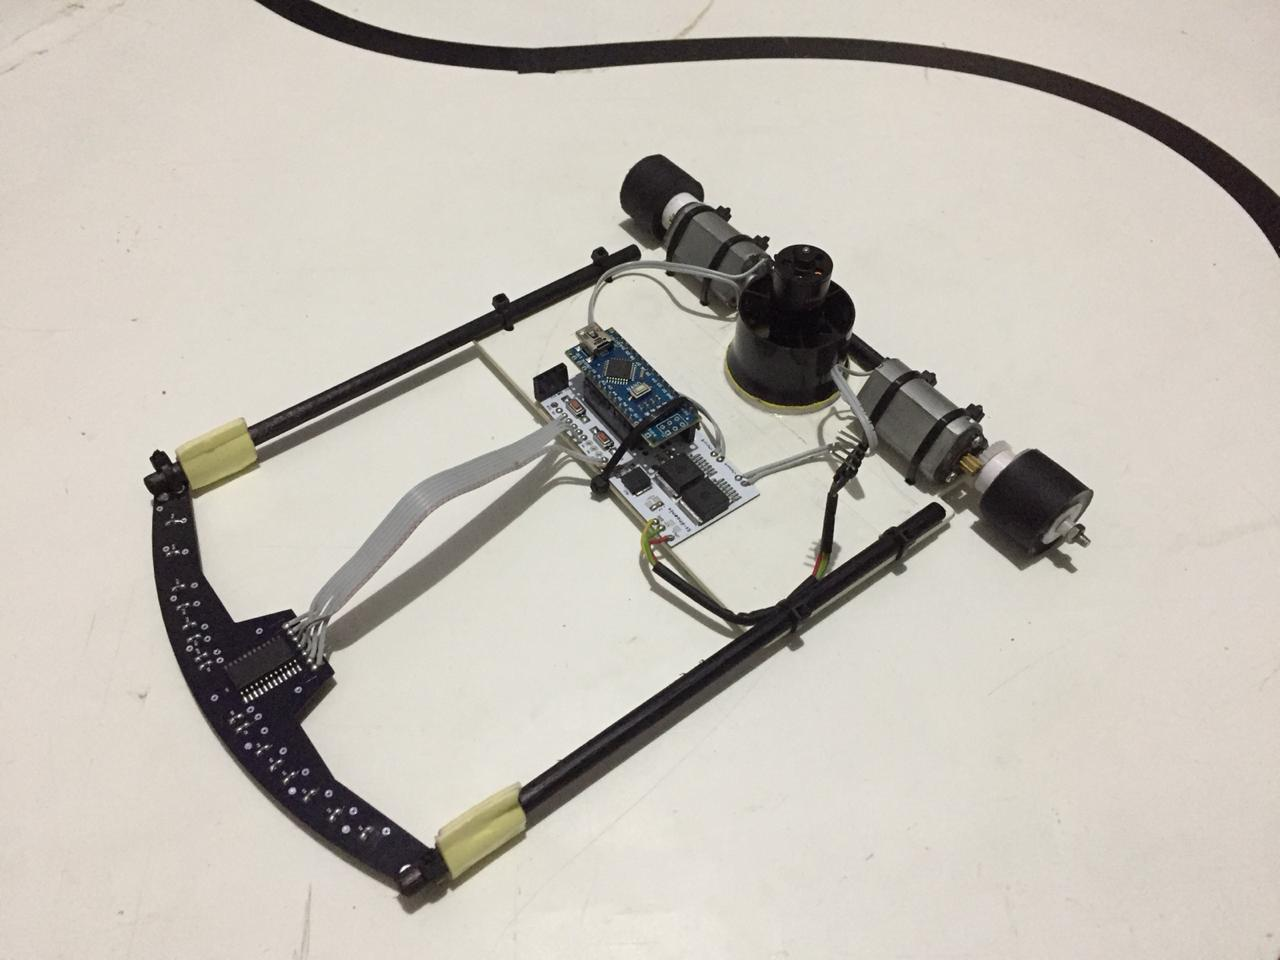
\includegraphics[width=0.5\linewidth]{img/image1.jpg}
    \caption{Seguidor de linea}
    \label{fig:enter-label}
\end{figure}


\section{Categorías en una competencia de seguidores de línea}

\subsection{Velocidad}

\begin{minipage}{0.4\textwidth}
    
        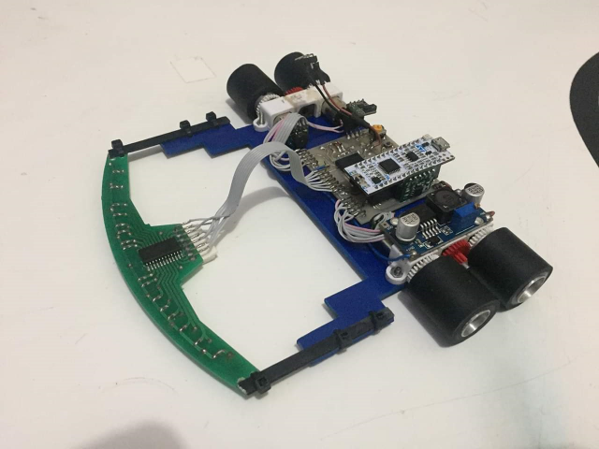
\includegraphics[width=\linewidth]{img/image2.png}
\end{minipage}
\hfill
\begin{minipage}{0.5\textwidth}
    Los robots compiten para completar una pista de línea (20 mm +- 5\%) en el menor tiempo posible.
Tres tipos:

\begin{itemize}
    \item Línea blanca sobre fondo negro.
	\item Línea negra sobre fondo blanco.
	\item Mixto. magnitudes físicas (temperatura, luminosidad, etc.)
\end{itemize}
\end{minipage}


\subsection{Precisión}

\begin{minipage}{0.4\textwidth}
    Esta categoría se enfoca en la precisión del seguimiento de línea. Los robots deben mantenerse lo más cerca posible de la línea y evitar desviaciones o errores. Se pueden utilizar diferentes métricas para evaluar la precisión, como la distancia promedio a la línea o el número de desviaciones cometidas.

\end{minipage}
\hfill
\begin{minipage}{0.5\textwidth}
    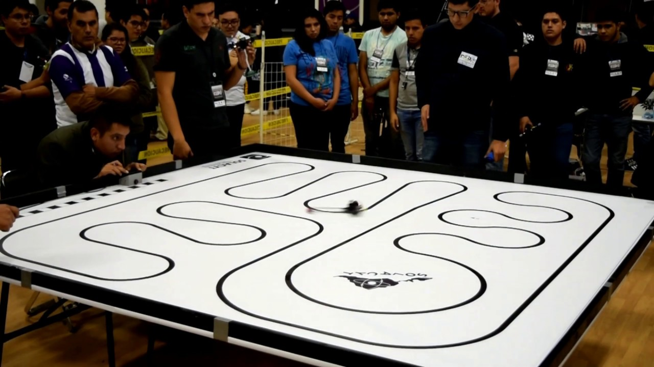
\includegraphics[width=\linewidth]{img/image3.png}
\end{minipage}


\subsection{Obstáculos}

\begin{minipage}{0.4\textwidth}
    
        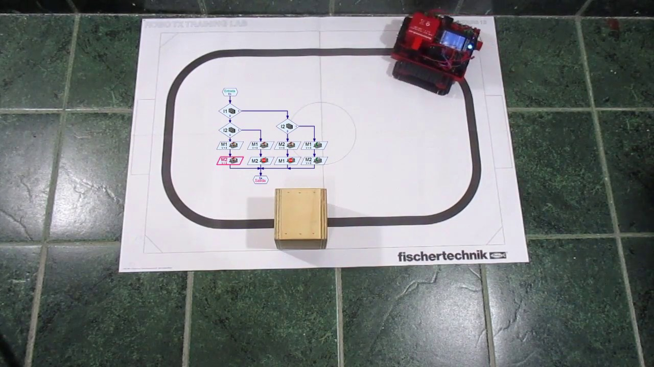
\includegraphics[width=\linewidth]{img/image4.png}
\end{minipage}
\hfill
\begin{minipage}{0.5\textwidth}
En esta categoría, los robots deben seguir la línea mientras sortean obstáculos en el camino. Los obstáculos pueden ser físicos, como paredes o barreras, o virtuales, como áreas de exclusión o zonas peligrosas. Los robots deben ser capaces de detectar y evitar los obstáculos de manera efectiva mientras siguen la línea

\end{minipage}


\subsection{Laberinto}

\begin{minipage}{0.4\textwidth}
    En esta categoría, los robots deben seguir una línea a través de un laberinto complejo. El desafío radica en la capacidad del robot para tomar decisiones en los cruces y encrucijadas del laberinto y encontrar la ruta correcta para seguir la línea hasta el final.


\end{minipage}
\hfill
\begin{minipage}{0.5\textwidth}
    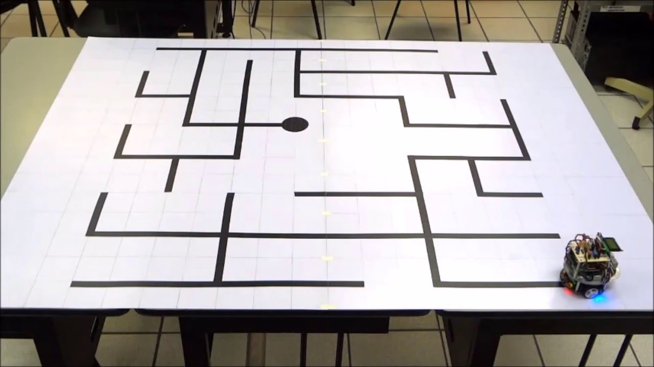
\includegraphics[width=\linewidth]{img/image5.png}
\end{minipage}

\section{Sensores para seguidores de línea}

\subsection{Sensor infrarrojo}

Está compuesto de un LED infrarrojo y un fototransistor, situados uno al lado del otro. El LED actúa como emisor y el fototransistor actúa como receptor. El LED infrarrojo emite luz infrarroja, es decir, de mayor longitud de onda (o menor frecuencia), invisible al ojo humano. 

Si esta luz choca contra una superficie blanca, se reflejará y rebotará hacia el fototransistor. En cambio, si choca contra una superficie negra, el material absorberá la mayoría de la luz y esta no llegará al fotorreceptor.

\begin{figure}[H]
    \centering
    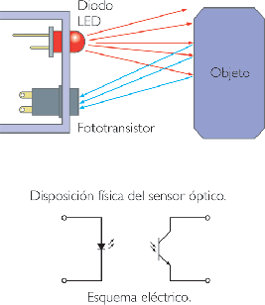
\includegraphics[width=0.3\linewidth]{img/image6.png}
    \caption{Fototransistor.}
    \label{fig:transistor-corte}
\end{figure}


\begin{figure}[H]
    \begin{subfigure}[t]{0.475\textwidth}
        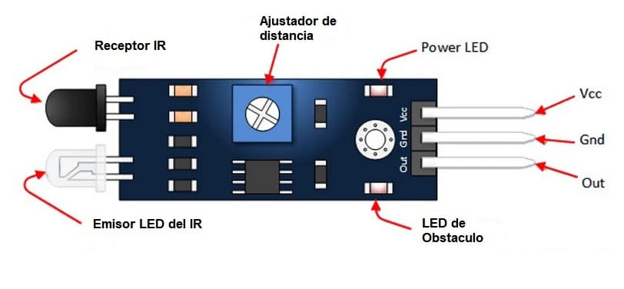
\includegraphics[width=1\textwidth]{img/image7.png}
        \caption{Driver sensor infrarrojo}
        \label{subfig:example-image-b}
    \end{subfigure}%
    \hfill
    \begin{subfigure}[t]{0.475\textwidth}
        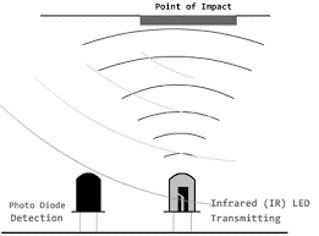
\includegraphics[width=1\textwidth]{img/image8.png}
        \caption{Funcionamiento de fotodiodo}
        \label{subfig:example-image-c}
    \end{subfigure}
    \caption{Sensor infrarrojo de Led}
    \label{fig:test_subfigure}
\end{figure}

\subsubsection{Diferencias}

Los fototransistores son similares a los fotodiodos excepto que si proporcionan amplificación a la corriente. Por lo general, se diseñan utilizando transistores NPN normales con su unión PN de colector-base expuesta a la luz a través de una carcasa o una lente transparentes. Entonces, son también de “tipo 2” como los fotodiodos, ya que no generan corriente en sé.

Debido a la amplificación de la corriente, su corriente de salida es de 50 a 100 veces mayor que la de los fotodiodos. Otra característica es que la región de la base está aislada eléctricamente o tiene control de sensibilidad.

Como el fototransistor ya proporciona amplificación de corriente, a diferencia de un fotodiodo, y no requiere amplificador externo para su funcionamiento. Un fototransistor es simplemente un transistor típico con un colector de base expuesto a la luz.


\begin{figure}[H]
    \begin{subfigure}[t]{0.475\textwidth}
        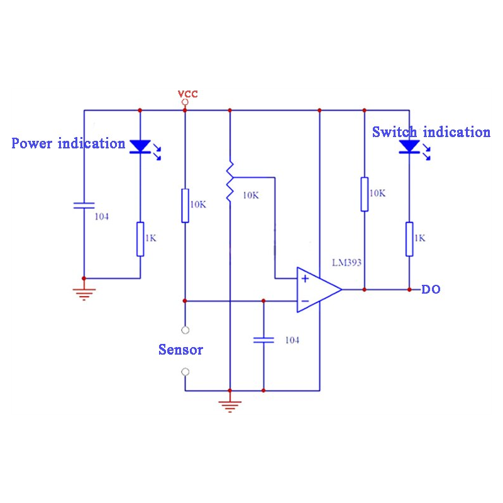
\includegraphics[width=1\textwidth]{img/image9.png}
        \caption{Driver sensor infrarrojo}
        \label{subfig:example-image-b}
    \end{subfigure}%
    \hfill
    \begin{subfigure}[t]{0.475\textwidth}
        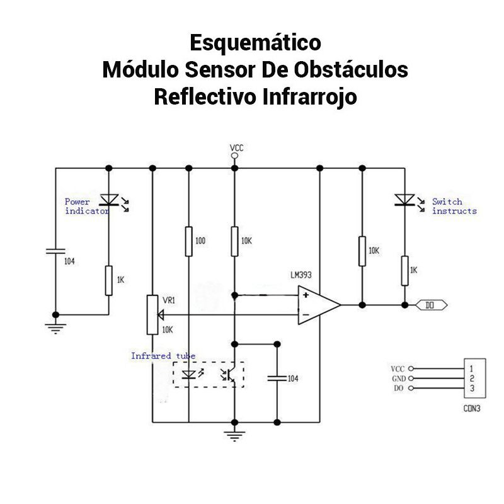
\includegraphics[width=1\textwidth]{img/image10.png}
        \caption{Funcionamiento de fotodiodo}
        \label{subfig:example-image-c}
    \end{subfigure}
    \caption{Sensor infrarrojo de Led}
    \label{fig:test_subfigure}
\end{figure}

\begin{figure}[H]
    \centering
    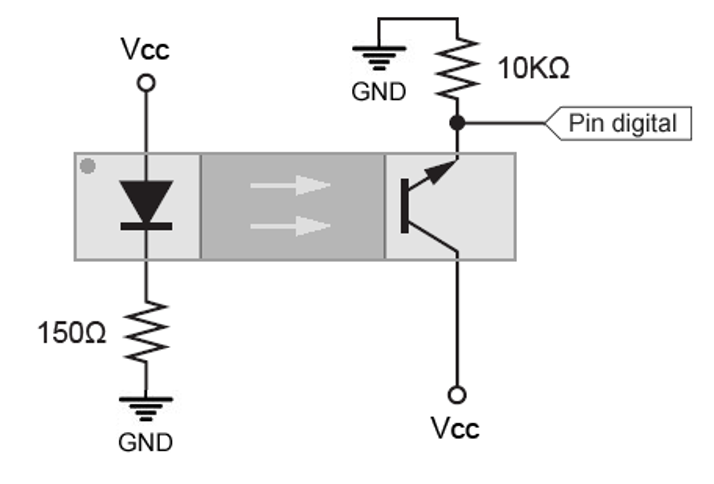
\includegraphics[width=0.6\linewidth]{img/image11.png}
    \caption{Fototransistor.}
    \label{fig:transistor-corte}
\end{figure}



\subsubsection{Sensores más usados}
\begin{figure}[H]
    \begin{subfigure}[t]{0.475\textwidth}
        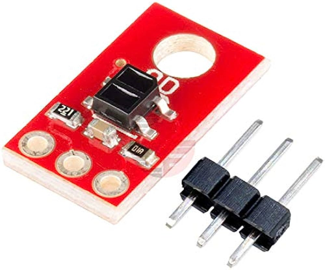
\includegraphics[width=1\textwidth]{img/image12.png}
        \caption{Driver sensor infrarrojo}
        \label{subfig:example-image-b}
    \end{subfigure}%
    \hfill
    \begin{subfigure}[t]{0.475\textwidth}
        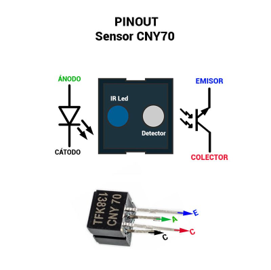
\includegraphics[width=1\textwidth]{img/image13.png}
        \caption{Funcionamiento de fotodiodo}
        \label{subfig:example-image-c}
    \end{subfigure}
    \caption{Sensor infrarrojo de Led}
    \label{fig:test_subfigure}
\end{figure}



\subsubsection{Regletas de sensores}


\begin{figure}[H]
    \begin{subfigure}[t]{0.475\textwidth}
        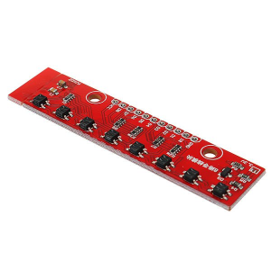
\includegraphics[width=\textwidth]{img/14.png}
        \caption{Simbolos}
        \label{subfig:example-image-b}
    \end{subfigure}%
    \hfill
    \begin{subfigure}[t]{0.475\textwidth}
        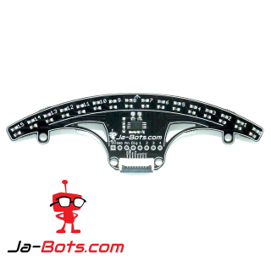
\includegraphics[width=\textwidth]{img/15.png}
        \caption{Potenciómetros}
        \label{subfig:example-image-c}
    \end{subfigure}

    \medskip % Agrega espacio vertical entre las filas de imágenes

    \begin{subfigure}[t]{0.475\textwidth}
        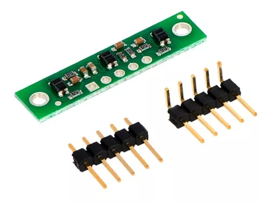
\includegraphics[width=\textwidth]{img/16.png}
        \caption{Potenciómetro tipo trimpot}
        \label{subfig:example-image-d}
    \end{subfigure}%
    \hfill
    \begin{subfigure}[t]{0.475\textwidth}
        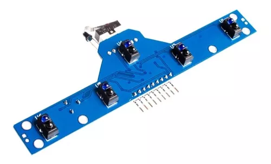
\includegraphics[width=\textwidth]{img/17.png}
        \caption{Potenciómetro tipo trimmer}
        \label{subfig:example-image-e}
    \end{subfigure}

    \caption{Tipos de resistencias variables}
    \label{fig:test_subfigure}
\end{figure}

\subsubsection{¿Qué pasa si tengo una regleta de 16 sensores y mi arduino nano no tiene 16 entradas analógicas? }

\begin{minipage}{0.4\textwidth}
    
        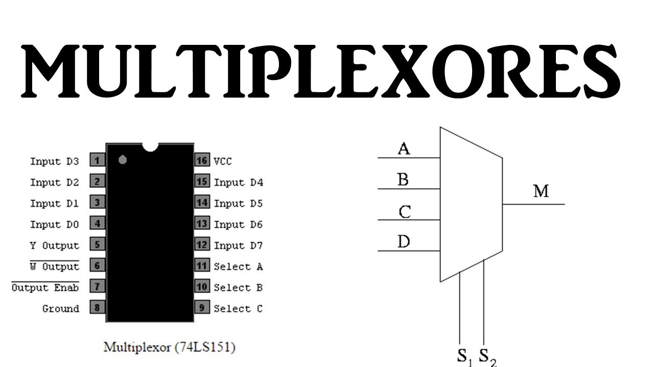
\includegraphics[width=\linewidth]{img/18.png}
\end{minipage}
\hfill
\begin{minipage}{0.5\textwidth}
Un multiplexor es un circuito digital que selecciona una de entre varias entradas de datos Ii y lleva su valor lógico a la única salida Z del circuito.

\end{minipage}

\begin{figure}[H]
    \centering
    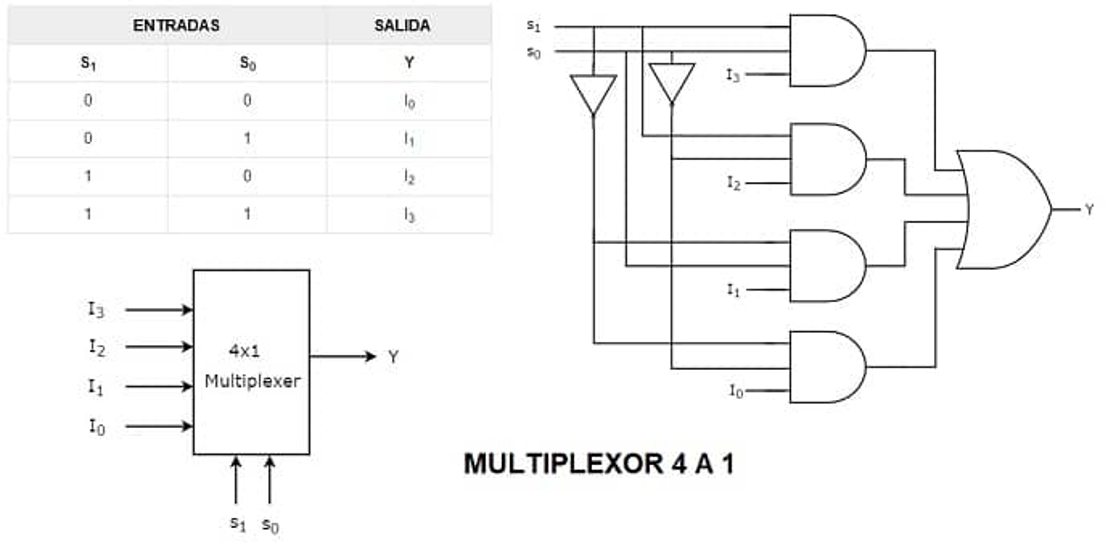
\includegraphics[width=0.7\linewidth]{img/21.png}
    \caption{Funcionamiento de multiplexor.}
    \label{fig:transistor-corte}
\end{figure}

\subsubsection{Sensores más usados}
\begin{figure}[H]
    \begin{subfigure}[t]{0.475\textwidth}
        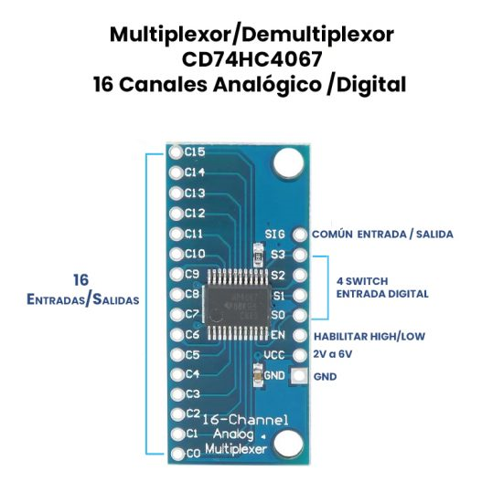
\includegraphics[width=1\textwidth]{img/19.png}
        \caption{Driver sensor infrarrojo}
        \label{subfig:example-image-b}
    \end{subfigure}%
    \hfill
    \begin{subfigure}[t]{0.475\textwidth}
        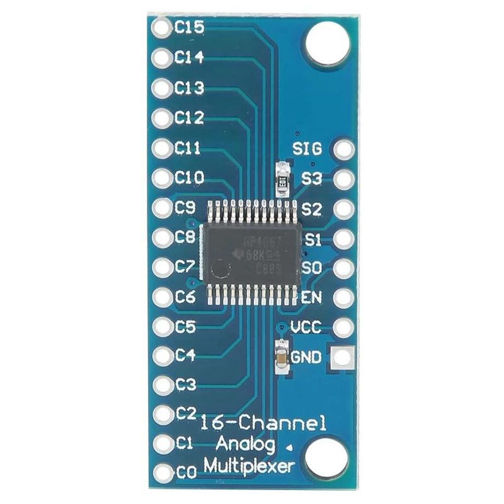
\includegraphics[width=1\textwidth]{img/20.png}
        \caption{Funcionamiento de fotodiodo}
        \label{subfig:example-image-c}
    \end{subfigure}
    \caption{Sensor infrarrojo de Led}
    \label{fig:test_subfigure}
\end{figure}

% ======================================== Fin Document ========================================



% ======================================== Début Annexes ========================================

\begin{appendices}

\chapter*{Tabla de anexos}
\startcontents[chapter]
\printcontents[chapter]{l}{0}{\setcounter{tocdepth}{3}}

\chapter{Primer anexo}

\cite{CitekeyBook}

\includepdf[pages=-,width=10cm]{example-image-a4}

\end{appendices}

% ======================================== Fin Annexes ========================================

\end{document}
